%!TEX root = thesis.tex

In this thesis we will introduce the notion of \emph{Ad Hoc Interfaces} or AHIs.

This chapter will contain our initial thoughts on AHIs and the directions we will take to explore the concept.
This initial presentation of the concept is based on the previous chapters where we take inspiration from various different fields and research areas to try and carve out our niche amongst the related computer science areas.

While this part is based on a theory approach we will, after this chapter, take a `research through design' approach where we study the field, make prototypes and evaluations to hopefully shed more light on the matter of AHIs and most likely re-evaluate parts of our initial thoughts and definitions, based on our prototyping and design experiences. 

\section{Defining Ad Hoc Interfaces}
Being \emph{ad hoc} generelly means something made for a specific task or creating meaning in changing contexts.
The word itself originates from the Latin language and literally means \emph{for this} (situation). 
In modern english the two word combination is regarded as a single word and the Oxford Dictionary\footnote{http://oxforddictionaries.com/definition/english/ad-hoc} defines it as

\begin{quotation}
\textbf{Ad hoc}  /ad 'h\textturnscripta k/

created or done for a particular purpose as necessary
\end{quotation}

The word is used in many different fields and context.
For example, In society committees a formed on an ad hoc basis to deal with specific tasks, investigations or analyses.

In computer science wireless networking can be of an ad hoc nature, which means that that the network is not dependent on a preexisting infrastructure.
Wireless ad hoc networks are highly dynamic and all participating nodes in the network graph are more or less doing routing for each other.
This makes the network adaptive to changing contexts, which is an important element of ubiquitous computing.

In general a user works with a computer in an ad hoc manner.
General purpose computers are very good at supporting ad hoc activities with their multitasking capabilities.
Applications are used when needed and maybe even used in connection with each other.
Windows are opened, closed and arranged as needed to support different use cases.

Even the TV industry is confronted with a change in demand.
Change in peoples TV viewing habits have made streaming services such Netflix, HBO etc. increasingly popular as they deliver content on demand.

So, ad hoc is a prevalent characteristic within many activities and contexts and we see a tendency in the digital world to allow for ad hoc interaction where to better accommodate the needs and wishes of the user.
The question is whether these qualities can be transferred into the world of physical objects and interfaces in a meaningful way, retaining the dynamic nature that is embedded in the definition of being ad hoc.

Next we will give our own definition of being ad hoc when applied to the field of physical user interfaces and also compare this to other parts of the HCI research area.

\subsection{Definition} 
We define ad hoc interfaces as 

\begin{quotation}\label{adhoc:definition}
\emph{physical interfaces that can be created or accessed on} 

\emph{demand for a particular purpose in mind. }
\end{quotation}

In this sense there is a degree of temporality embedded in the definition, in that the interaction is somewhat impromptu and the purpose is non-continuing.
The interface can be accessed when needed and when the interaction and purpose has ended it ``disappears'' again, for example by slowly letting it perish when it is no longer used, either manually, over time, by natural forces or based on sensory data.
This makes good sense in the digital realm as pixels on a screen can easily be controlled and abstracted to bring attention to different tasks.
The questions is, how do we apply these ad hoc elements or characteristics to physical interfaces.
The physical world comes with many constraints compared to the digital as we are limited by the characteristics of the materials we interact with and the general laws of physics.
We can't just magically make physical objects appear and disappear which is possible, and easy, to do on a digital display.

\todo{mere her}

We have identified three overall approaches to creating physical interfaces with ad hoc capabilities that we would like to explore through prototyping.

\begin{enumerate}
	\item{Using shape change as the construction mechanism}
	\item{Through invisible interfaces embedded into the physical environment}
	\item{Literally constructing the interface on the spot}
\end{enumerate}

The three approaches do not exclude each other as they could surely be combined while still living up to our definition.
In the following we will elaborate on our initial thoughts for each approach while we in chapters~\autoref{ch:jamming}--\ref{ch:prototype3}  explore each of the three approaches in a prototyping context.
 
\begin{verbatim}
introducerer muligheden for baade space- og time multiplexing??
\end{verbatim}

\subsubsection{Using shape change as the construction mechanism}
To adhere to the dynamic nature that we propose for AHIs, using shape change is a particular drawing approach to creating such interfaces.
In this case an objects shape changing capabilities lets it shift or morph into an particular interface with an accompanying set of functions, as form becomes function.
The interface can either be changed by the user to suit a particular task or need, or by the computer in relation to changes to its digital state or as response to a user action.
To control the change of shape sensors and actuators would be embedded for input and output control.

Affordances are to a large extend dictated by the perceived action possibilities of the particular end-shape or the transition-phase into the end-shape and are therefore changing as the interface changes shape and function.

In \autoref{ch:jamming} we explore this approach.

\subsubsection{Embedding invisible interfaces into the physical environment}
In this case an existing element of the environment will contain the interface.
An element can be both a physical object, for example walls, furniture, devices etc., and also the ambient air \todo{there is a better word for this} that surrounds us.
By embedding the interface into existing objects the object itself will retain its normal function while the interface is inactive, while the augmented interface will be active when needed. 
The wall, for example, will still look and feel like a wall and retain its perceived affordances when the interface is inactive, but will gain additional functions when the interface is needed by the user.
In this sense the interface is invisibly embedded into the environment until it is needed.

The perceived action possibilities of the interface will be somewhat constrained by the affordances of the object which might be a challenge, depending on the intended use of the system.
Where a wall might invite to be used as a touch surface it does not really invite to be used as a drum, as a pillow might do.

The input and output possibilities will also depend on the materiality of the physical object as they are closely tied together but we envision that a variety of sensors and actuators can be used for input and output.

In \autoref{ch:textile-touch} we explore this approach.

\subsubsection{Constructing the interface on the spot}
This approach originated from the idea of interfaces that was ``fashioned from whatever is immediately available''.
While this may not be quite possible, the idea is engaging and intriguing as an embodiment of a very literal version of AHIs.

Here we envision an approach to AHIs where the actual interface is constructed on the spot in a quick to make, quick to erase fashion.
By using special materials, the form or composition of the constructed interface will define the associated functions.
Again, this is an attempt to bring out digital qualities into the physical space as this construction of physical interfaces in a sense becomes a kind of physical programming.
An approach like this is of course very restricted by the available materials, but also the fact that if we really want these interfaces to be quick to make, then the functions will be equally simple.
Though like in normal programming, layers of abstraction could provide advanced capabilities but maybe at the cost of unnecessary complexity or at the cost of less flexibility.

This approach is on our part the least explored of the three as it is has proven to be difficult with the materials of today, at least in the manifestation that was our initial point of origin. 

In chapter \ref{ch:prototype3} we explore this approach.

\subsection{Ad hoc characteristics in existing interfaces}
Ad hoc characteristics in interfaces are not some novel invention and they an be found in several existing products.
A simple example would be The Clapper\footnote{http://en.wikipedia.org/wiki/The\_Clapper} (figure~\ref{ch:adhoc:theclapper}) from the mid eighties, an electrical switch reacting to sounds in a specific frequency, tuned to claps, to turn a switch on and off respectively.
Here the interface is pervasive in the nearby environment and one interacts with it when needed after which it ``disappears'' again.

\begin{figure}[h]
	\centering
	\begin{minipage}[b]{.7\textwidth}
		\centering
		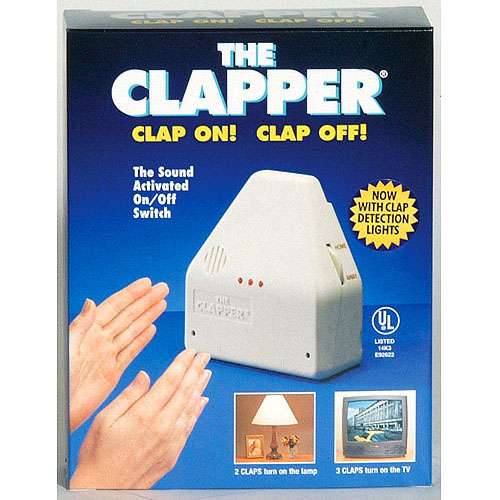
\includegraphics[width=.5\linewidth]{figures/theclapper}
		\caption{The Clapper, a sound activated electronic switch.}
		\label{ch:adhoc:theclapper}
	\end{minipage}
\end{figure}

Another example is the conceptual and somewhat futuristic product ShapePhone (figure~\ref{fig:ch:jamming:jui-phone}) based on particle jamming, which will also be addressed in \autoref{ch:jamming}.
ShapePhone is generic shape changing product which changes it behaviour based on its physical form.
For example, in its base form it is a phone but when wrapped around a wrist it could serve as a watch and when folded in some other way it could be a game controller.
So, the different interfaces are created on demand by the user and have very different purposes of use depending on the form of the interface.

\todo{afslut afrunding}.
\blank
\todo{2-3 flere eksempler \dots} 

\subsection{Relationship with other fields} 
% CAC comparison
It might seem that AHI overlaps with the concept of Context Aware Computing in that they both have a focus on environmental context.
In context aware computing a system attempts to derive, through a variety of cues, what the current context of use is and as a result it adapts its behaviour \citep[chap. 8]{krumm2009ubiquitous}. 
In this way it is the system itself that takes action autonomously while the user continues on, outside of the control loop.
Exactly the topic of control is one of the points where context aware systems have received criticism \cite{erickson2002some}, \citep[chap. 8]{krumm2009ubiquitous}.
The criticism has to do with a systems ability to make inference based on the analysis of quantitative contextual information available, something that can be quite difficult to do for a computer as contextual information is often subtle and implicit.
As such there is a possibility for a mismatch between the user and the computers inference of a situation leading to conflicts.
This is not to say that context aware systems are not useful or appropriate in some situations as they can offer a lot of convenience, if done with care and with the \emph{user} in mind, with all the complexity that follows it.

An aspect of our AHI definition is \emph{on-demand} where the word \emph{demand} both implies a concious and specific need and an explicit interaction.
This puts a focus on the user as the initiator of action and as such this might seem conflicting with context aware systems where the focus often is on implicit and autonomous actions.
But this does not mean that context-aware systems and AHIs necessary are incompatible, since they are both elements or characteristics of a system and one does not exclude the other as a part of a complex system.

It would seem quite natural to have an ad hoc system that also incorporates some context aware computing elements, as long as it does not put the user out of the control loop.
An example could be to use context information to identify which user is currently using the interface, enabling customizable profiles or actions to the specific users, but without letting the system take action or determine the most proper action for the user.
As with any successful context system this does however require reliable context information and a high degree of robustness to avoid it being a hindrance for the user experience.
\blank
% TUI comparison
Tangible user interfaces, or TUIs, do generally not exhibit ad hoc characteristics. \todo{compare to ambient tangibles}
They are mentioned here more for their nature of physical representation and their movement away from the standard GUI paradigm for human-computer interaction.
TUIs demonstrate a inherently tight coupling between digital information and the associated physical representation, for example tangible tokens representing a \emph{specific} digital entity or mapping to a \emph{specific} function or action.
There are numerous examples of these, for example, the ReacTable \cite{jorda2007reactable}, the Marble Answering Machine \todo{citation possible or link} to name a few.
Furthermore, because of this tight coupling the physical representations are often created only for the specific purpose and are of no use outside of the TUI context. \todo{giv evt. eksempel}

In contrast, ad hoc interfaces define a less strict coupling between digital content and physical objects, meaning that one physical object can serve several purposes.
This will be exemplified in \autoref{ch:textile-touch} where we prototype a general purpose ad hoc interface called Textile Touch, which can augment existing household objects by adding a digital layer. \todo{overvej lige hvordan det bliver augmented}
\blank
Shape-changing interface have indeed been an inspiration to our notion of AHIs as shape-change is an obvious construction approach to building such interfaces.
The dynamic nature of SCIs does well in supporting some of the properties of AHIs such as adaptability, malleability and a dynamic relationship between the physical and digital state of the interface.
This does not mean that SCIs are, per definition, AHIs, as the purpose of an SCIs does not necessarily match the user focus and \emph{on-demand\'ness} and \emph{ad hoc'ness} that we envision in AHIs.
Also AHIs are not, as can also be seen in our three proposed construction approaches, limited to the use of shape-change for implementing such interfaces.  

\section{Summary}

In this chapter we have given an introduction to ad hoc interfaces, a \todo{design approach} to user interfaces where the temporality of interaction is taken into account in the interface itself, and where the user is the initiator of action.
We have \todo{discussed} how AHIs relate to established fields of research and how the \todo{design approach} brings together different aspects of various fields within HCI.
Last but not least, we have identified three approaches to approaching AHIs that will be the guideline for our further explorations throughout this thesis.

As an opening to our explorations of AHIs and as an ending to this chapter, we would like to start off with a review of a preceding project we made in a course at Aarhus Univerity that in many ways have motivated our initial ideas about AHIs.

\section{Preceding project: BeoMotion}

The project that we would like to \todo{review} was made during a masters course in 2011 called Innovation Project\footnote{https://services.brics.dk/java/courseadmin/Inno\_pro2011}.
The course was provided in cooperation with the danish design company B\&O\footnote{http://www.bang-olufsen.com/} and the goal was to create novel concepts for B\&O for the purpose of unveiling technical, design and commercial potentials within home-automation systems.

Our contribution was the concept BeoMotion, a dynamic shape shifting wall module with the ability to change its surface structure for acoustic regulation, i.e. diffusion, absorption and reflection for optimal conditions \cite{beomotionreportstefan, beomotionreporttore}, see figure~\ref{fig:beomotion}.
The idea for the module was to retain the aesthetics of existing surroundings, so if the module was not in use, it would be ``invisible'' and flat like the wall (figure~\ref{fig:beomotion:concept_flat}).  
The acoustic functionality and the aesthetics that follow were the primary features of the modules.
Secondary, the modules had illumination features integrated into the modules.
In this way different areas of the modules could light up, both on the front (figure\ref{fig:beomotion:concept_light}) and as backlighting (figure~\ref{fig:beomotion:concept_backlight}), and serve as an aesthetic lighting for the atmosphere of the room.

We envisioned two scenarios of use for the wall.
One where context awareness was the primary driver which meant that everything (acoustic and lighting conditions) would be automatically sensed and the wall module would modify itself accordingly and shift from flat to actively in motion.
In the other scenario the user would, to a higher degree, be in control.
The user could actively create deformations on the surface for aesthetic purposes and also control illuminated areas by interacting with the wall surface, see figure~\ref{fig:beomotion:concept_backlight}.
In this scenario the interface was shaped and created by the user for the specific situation, i.e. current acoustic and lightning conditions, as well as the desired aesthetic expression. 

This project has spurred our initial thoughts on ad hoc interfaces though the notion of ad hocness was not deliberate at the time.
The ad hoc characteristics are \todo{twofold}.
Firstly, the acoustic features are hidden when not needed and then highly \todo{prevalent} when active as the otherwise static nature of walls start going in motion providing a engaging aesthetic expression.
Secondly, by using the surface of the wall as an interface in itself to control lighting conditions of the room. \todo{mere?}
Both are examples of addressing the second approach we earlier labeled 

\begin{quotation}
	\emph{Through invisible interfaces embedded into the physical environment}.
\end{quotation}

\begin{figure}[ht]
	\centering
	\begin{subfigure}{.45\textwidth}
		\centering
		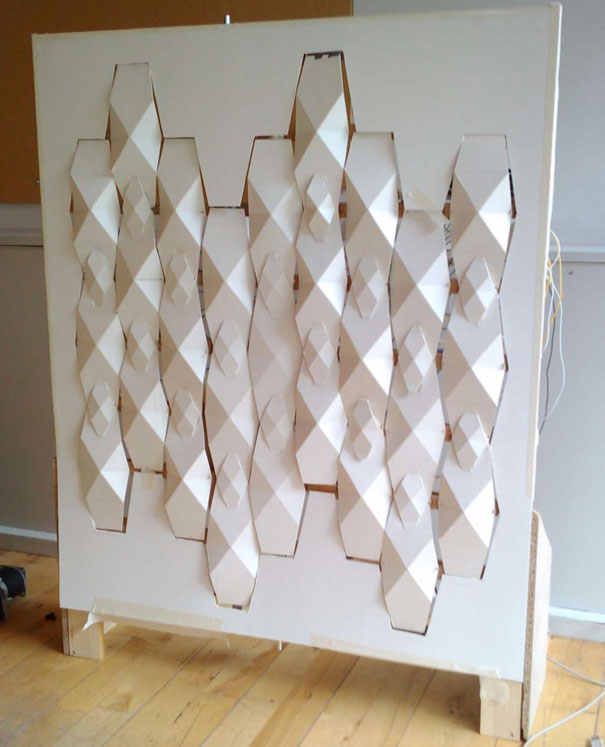
\includegraphics[width=\linewidth]{figures/beomotion/prototype_front}
		\caption{The interactive prototype (front). Made with a wooden framework and thick white cardboard with cuts for flexibility.}
		\label{fig:beomotion:proto_front}
	\end{subfigure}%
	\hspace{0.1cm}
	\vspace{0.5cm}
	\begin{subfigure}{.45\textwidth}
		\centering
		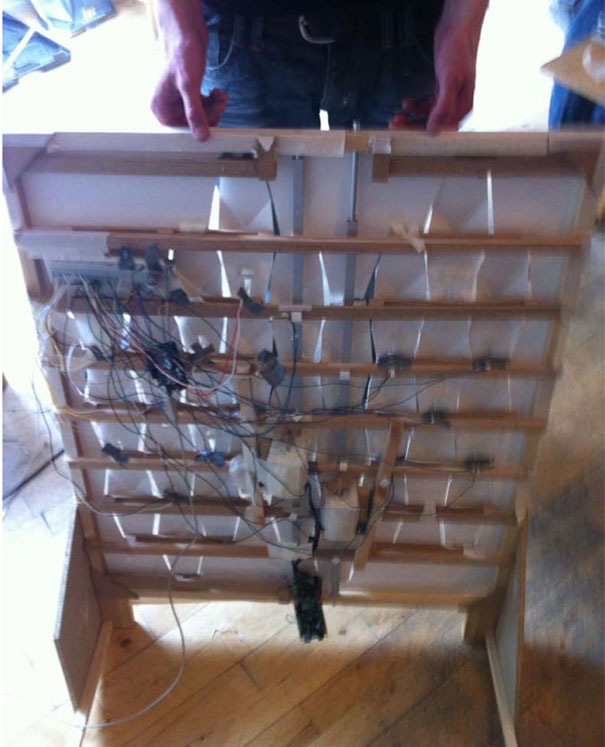
\includegraphics[width=\linewidth]{figures/beomotion/prototype_back}
		\caption{The interactive prototype (back). Arduino controlled LEDs and DC motors driving several fishing lines that pulling the cardboard shapes.}
		\label{fig:beomotion:proto_back}
	\end{subfigure}
	\vspace{0.5cm}
	\begin{subfigure}{.45\textwidth}
		\centering
		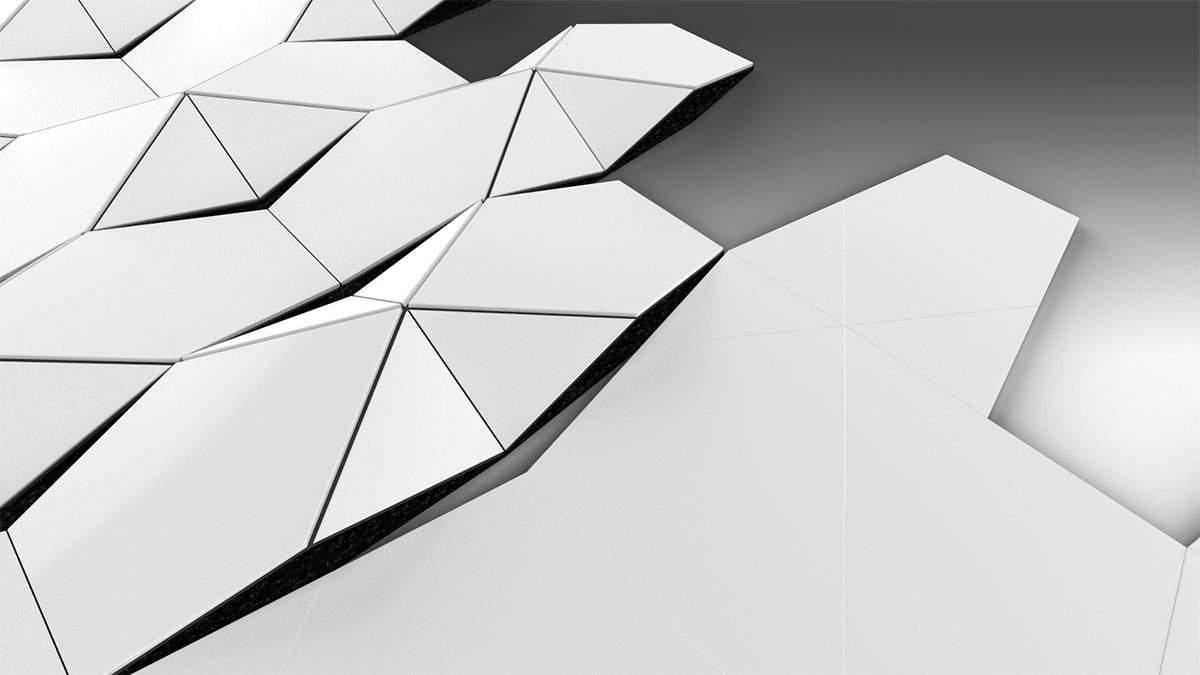
\includegraphics[width=\linewidth]{figures/beomotion/concept}
		\caption{A concept illustration of the dynamic shapes.}
		\label{fig:beomotion:concept}
	\end{subfigure}%
	\hspace{0.1cm}
	\begin{subfigure}{.45\textwidth}
		\centering
		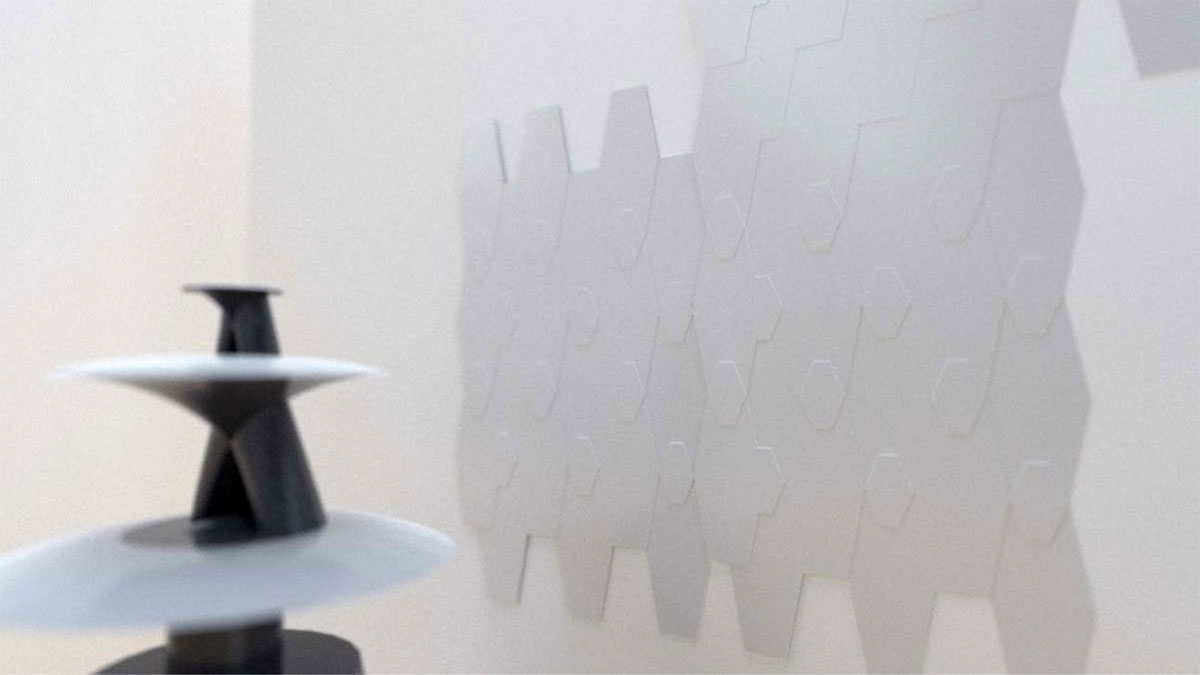
\includegraphics[width=\linewidth]{figures/beomotion/concept_flat}
		\caption{Illustration of the concept in flat state.}
		\label{fig:beomotion:concept_flat}
	\end{subfigure}
	\begin{subfigure}{.45\textwidth}
		\centering
		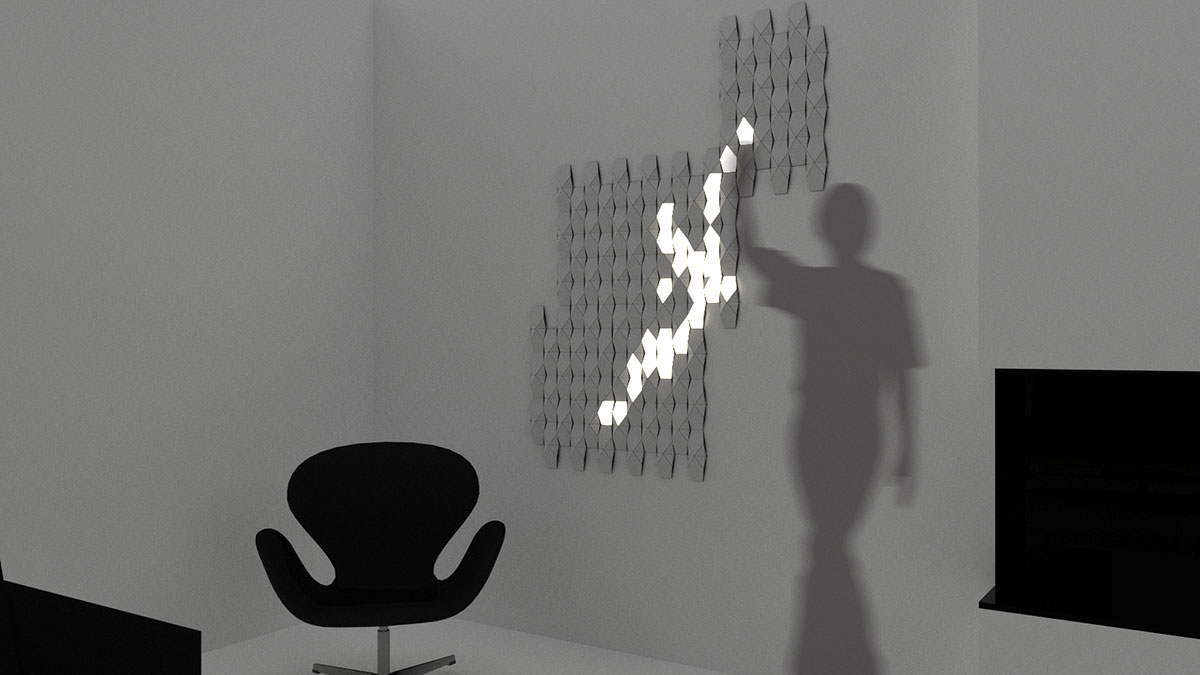
\includegraphics[width=\linewidth]{figures/beomotion/concept_lighting}
		\caption{Concept illustration of interaction with the illumination feature.}
		\label{fig:beomotion:concept_light}
	\end{subfigure}%
	\hspace{0.1cm}
	\begin{subfigure}{.45\textwidth}
		\centering
		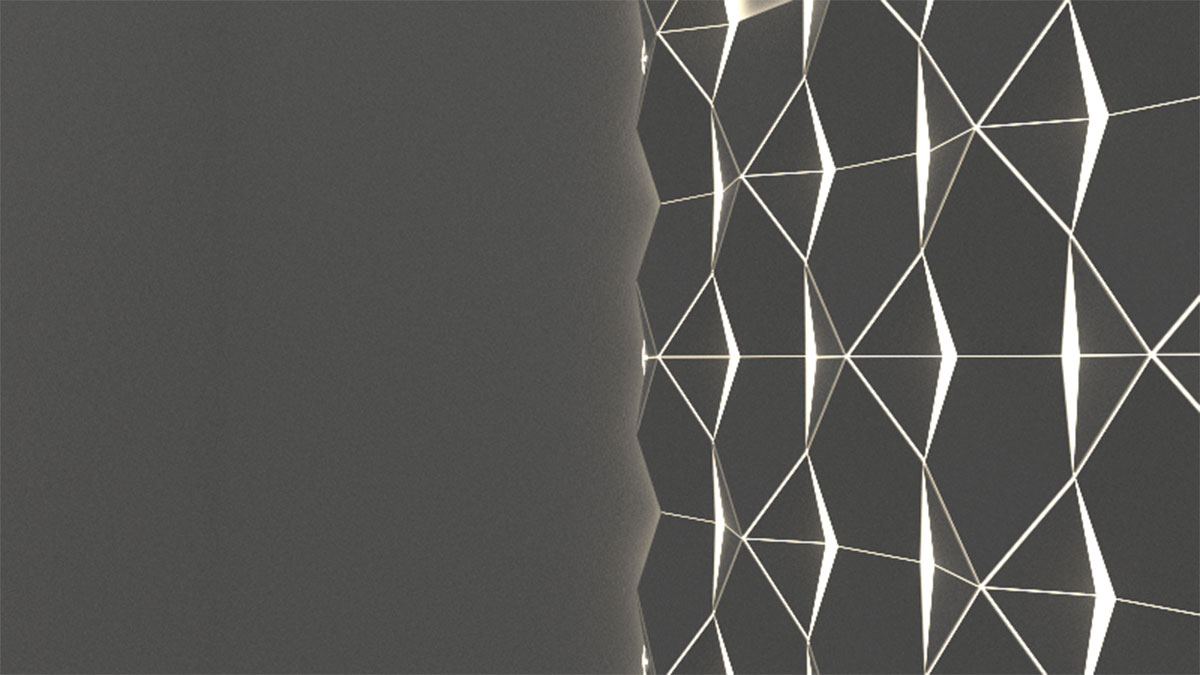
\includegraphics[width=\linewidth]{figures/beomotion/concept_backlight}
		\caption{Concept illustration of the backlighting feature.}
		\label{fig:beomotion:concept_backlight}
	\end{subfigure}
	\caption{BeoMotion product design, Innovation Project, Aarhus University 2011}
	\label{fig:beomotion}
\end{figure}
